\noindent
\textbf{CS4268 AY2025-26 Sem 2}
\\
\noindent
Lecturer: Divesh Aggarwal
\hfill
Lecture 3                      %%% FILL IN LECTURE NUMBER HERE
\hfill
Date: January 29, 2026          %%% FILL IN LECTURE DATE HERE


\noindent
\rule{\textwidth}{1pt}

\medskip

\section{Composite Systems}
We have discussed how to describe a single quantum system via the notion of quantum states residing in a Hilbert space, how they can be transformed and how information is extracted from the system via measurements. Now we discuss how to characterize \textit{composite} systems. Given two (or more) quantum systems, each with its own Hilbert space, how do we describe them collectively as a whole? In particular, if we only effect changes on a component of this composite system, how can we describe this mathematically as an operation on the entire system? 

This is achieved via the notion of \textit{tensor products}.

\subsection{Tensor Products}
Let us consider a system comprising simply two qudits. This system is mathematically described by the tensor product of the Hilbert spaces of the individual qudits:

\begin{definition}[Tensor Product of Hilbert Spaces]\label{definition:tensor_products}
    Given two qudit Hilbert spaces $\mathcal{H}_1 = \mathbb{C}^{d_1}$, $\mathcal{H}_2 = \mathbb{C}^{d_2}$ spanned respectively by the computational basis vectors
    \[
    \mathcal{B}_1 = \{\ket{0}, \ket{1}, \dots, \ket{d_1-1}\}, \quad 
    \mathcal{B}_2 = \{\ket{0}, \ket{1}, \dots, \ket{d_2-1}\},
    \]
    the \textbf{tensor product} of $\mathcal{H}_1$ and $\mathcal{H}_2$ is defined as the Hilbert space
    \[
    \mathcal{H}_1 \otimes \mathcal{H}_2 = \text{span} \{\ket{i} \otimes \ket{j} : 0 \le i \le d_1-1, 0 \le j \le d_2-1 \}.
    \]

    Each (normalized) state $\ket{\psi} = \sum_{ij} {a_{ij}}\ket{i} \otimes \ket{j} \in \mathcal{H}_1 \otimes \mathcal{H}_2$, $\sum_{ij}|a_{ij}|^2=1$, is a legitimate characterization of the entire system. Also, for brevity we shall henceforth write $\ket{\alpha} \otimes \ket{\beta}$ simply as $\ket{\alpha\beta}$.

    More generally, for $n>2$ systems, the tensor product generalizes naturally to
    \[
    \mathcal{H}_1 \otimes \mathcal{H}_2 \otimes \dots \otimes \mathcal{H}_n = \text{span}\{\ket{i_1}\otimes \dots \otimes \ket{i_n}\}.
    \]
\end{definition}

\begin{remark}[Existence and Uniqueness of Tensor Products]
    Note that above we have defined the tensor product as being the span of the \textit{formal} symbols $\ket{i} \otimes \ket{j}$ -- we have not at all dissected what the symbols $\ket{i} \otimes \ket{j}$ really mean. In particular, what is the difference between $\ket{i} \otimes \ket{j}$ and the \textit{direct sum} $(\ket{i}, \ket{j})$? Superficially, both seem quite similar in the sense that the individual constituents are simply concatenated together (albeit in different notations). Indeed, these two notions are closely related: roughly speaking, we think of the symbol $\otimes$ as a \textit{bilinear map} from the direct sum/Cartesian product $H_1 \times H_2$ to the Hilbert space $Z$ (we use the symbol $Z$ because we have not yet proved that this thing exists). That is, the purported map $\otimes$ behaves as such (on all vectors $\ket{u}, \ket{v}$, not just the basis vectors):
    \begin{align*}
        \otimes(\ket{u},\ket{v}) := \ket{u} \otimes \ket{v}
    \end{align*}
    such that
    \begin{align}\label{equation:tensor_product_multilinearity}
        (a\ket{u_1}+b\ket{u_2}) \otimes \ket{v} &= a\ket{u_1} \otimes \ket{v} + b\ket{u_2} \otimes \ket{v}\\
        \ket{u} \otimes(a\ket{v_1}+b\ket{v_2}) &= a\ket{u} \otimes \ket{v_1} + b\ket{u} \otimes \ket{v_2}.
    \end{align}
    The existence and (essential) uniqueness of the map $\otimes$ is nontrivial to show. Once these are taken care of we can start calling $Z$ as $H_1 \otimes H_2$. If you are interested, the wiki article on \href{https://en.wikipedia.org/wiki/Tensor_product}{tensor products} is a good starting point. Be warned however that this leads to a long rabbit hole.

    That was a lot of yapping -- but we won't worry about any of that in this course. In practice, think of $\otimes$ as concatenation plus multilinearity: the symbol $\otimes$ is used to stack different basis vectors from different Hilbert spaces together, and that $\otimes$ is linear with respect to \textit{all} its arguments, i.e. \cref{equation:tensor_product_multilinearity}
\end{remark}

\begin{fact}[Column Vector Representation of Tensor Products]
    Given vectors $\ket{\alpha} \in \mathcal{H}_1$ and $\ket{\beta} \in \mathcal{H}_2$, the column representation of $\ket{\alpha}\otimes \ket{\beta}$ is given by
    \begin{align*}
        \ket{a} \otimes \ket{b} = \begin{pmatrix} a_0 \\ \vdots \\ a_{d_1-1} \end{pmatrix} \otimes \begin{pmatrix} b_0 \\ \vdots \\ b_{d_2-1} \end{pmatrix} = \begin{pmatrix} a_0 b_0 \\ \vdots \\ a_0 b_{d_2-1} \\ \vdots \\ a_{d_1-1} b_{0} \\ \vdots \\ a_{d_1-1} b_{d_2-1} \end{pmatrix}.
    \end{align*}
    In particular, the tensor product of the basis vectors is given by
    \[
    \ket{i} \otimes \ket{j} =
    \begin{bmatrix}0 \\ \vdots \\ 1 \\ \vdots \\ 0 \end{bmatrix}
    \]
    where the $1$ appears at position $i \cdot d_2 + j$.
\end{fact}
These results are immediate from the definition of the tensor product.

\begin{example}
    For two qubits ($d_1 = d_2 = 2$), the computational basis states are represented as
    \[
    \ket{0} = \begin{bmatrix}1\\0\end{bmatrix}, \qquad
    \ket{1} = \begin{bmatrix}0\\1\end{bmatrix}.
    \]
    The superposition states are
    \[
    \ket{+} = \frac{1}{\sqrt{2}}\begin{bmatrix}1\\1\end{bmatrix}, \qquad
    \ket{-} = \frac{1}{\sqrt{2}}\begin{bmatrix}1\\-1\end{bmatrix}.
    \]
    
    We now give examples of tensor products in column-vector form:
    \begin{align*}
    \ket{0}\otimes\ket{0}
    &=
    \begin{bmatrix}1\\0\\0\\0\end{bmatrix},\\[6pt]
    \ket{0}\otimes\ket{+}
    &=
    \frac{1}{\sqrt{2}}
    \begin{bmatrix}1\\1\\0\\0\end{bmatrix},\\[6pt]
    \ket{+}\otimes\ket{0}
    &=
    \frac{1}{\sqrt{2}}
    \begin{bmatrix}1\\0\\1\\0\end{bmatrix},\\[6pt]
    \ket{+}\otimes\ket{-}
    &=
    \frac{1}{2}
    \begin{bmatrix}1\\-1\\1\\-1\end{bmatrix}.
    \end{align*}

    More generally, suppose Alice has qubit $\ket{A} = \alpha_0\ket{0} + \alpha_1\ket{1}$ and Bob has qubit $\ket{B} = \beta_0\ket{0} + \beta_1\ket{1}$. Then their joint state is
    \[
    \ket{A}\otimes\ket{B} = \alpha_0\beta_0 \ket{0}\otimes\ket{0} + \alpha_0\beta_1 \ket{0}\otimes\ket{1} 
    + \alpha_1\beta_0 \ket{1}\otimes\ket{0} + \alpha_1\beta_1 \ket{1}\otimes\ket{1}.
    \]
    Notice how the multilinearity (bilinearity here) was invoked to obtain this expansion. In column vector form:
    \[
    \ket{A}\otimes\ket{B} =
    \begin{bmatrix}
    \alpha_0\beta_0 \\ \alpha_0\beta_1 \\ \alpha_1\beta_0 \\ \alpha_1\beta_1
    \end{bmatrix}.
    \]
    To verify that the composite coefficients are indeed probability amplitudes, we check if the sum of amplitudes squared is 1. But this is easy -- according to Quantum Mechanics Law 1, the amplitudes of $\ket{A}$ and $\ket{B}$ satisfy the \textbf{normalization condition} i.e. $|\alpha_0|^2 + |\alpha_1|^2 = 1$ and $|\beta_0|^2 + |\beta_1|^2 = 1$, so
    \begin{align*}
    |\alpha_0\beta_0|^2 + |\alpha_0\beta_1|^2 + |\alpha_1\beta_0|^2 + |\alpha_1\beta_1|^2
    &= |\alpha_0|^2(|\beta_0|^2 + |\beta_1|^2) + |\alpha_1|^2(|\beta_0|^2 + |\beta_1|^2)\\
    &= |\alpha_0|^2 + |\alpha_1|^2\\
    &= 1
    \end{align*}
    as desired.
\end{example}

\begin{definition}[Tensor Product of Matrices]
    Given matrices $A \in \mathbb{C}^{m\times n}$ and $B \in \mathbb{C}^{p\times q}$, their tensor (also called Kronecker) product $A \otimes B$ is the $mp \times nq$ matrix
    \[
    A \otimes B =
    \begin{bmatrix}
    a_{11}B & a_{12}B & \cdots & a_{1n}B \\
    a_{21}B & a_{22}B & \cdots & a_{2n}B \\
    \vdots & \vdots & \ddots & \vdots \\
    a_{m1}B & a_{m2}B & \cdots & a_{mn}B
    \end{bmatrix}.
    \]
\end{definition}

\begin{remark}
    We seem to have two different (but superficially very similar) notions of tensor products, one for vectors and one for matrices, but note that technically the set of matrices itself is an abstract vector space, thus there really is no difference on an abstract level. The only difference here of course is the \textit{concrete representation} of the objects. What we call vectors in this course we generally write down as columns (long-ish 1D objects), while the operators on these vectors (which technically speaking also form a vector space themselves) we write down as matrices (square-ish 2D objects). Hopefully this isn't too confusing. If it helps you can restack the rectangular-looking matrices into long columns (vectorization). Then the basis matrices spanning matrix space gets rewritten as long, all-zeros-except-one vectors. Then this should be very clear that the tensor product of matrices is exactly the same as the general definition given in \cref{definition:tensor_products}.
\end{remark}
 

\begin{proposition}
The tensor product of matrices satisfies the following properties:
\begin{itemize}
    \item $(A \otimes B)(C \otimes D) = (AC) \otimes (BD)$ whenever dimensions match.
    \item $(A \otimes B)^\dagger = A^\dagger \otimes B^\dagger$.
    \item $\mathrm{Tr}(A \otimes B) = \mathrm{Tr}(A)\mathrm{Tr}(B)$.
    \item If $A$ and $B$ are invertible, then $(A \otimes B)^{-1} = A^{-1} \otimes B^{-1}$.
\end{itemize}
\end{proposition}

Why are matrix tensor products useful? Recall that matrices appear a lot in quantum, as operations on the quantum states (unitaries, measurements etc). Matrix tensor products characterize the \textit{joint} application of these operations on the entire system. Consider a two qubit basis state $\ket{\psi}=\ket{00}$. Suppose we apply a unitary transformation $U= \begin{bmatrix} p & r \\ q & s \end{bmatrix}$ only to the second qubit.

The overall transformation on $\ket{\psi}$ can be described by
$$
    \ket{00} \rightarrow \ket{0} \otimes (U\ket{0})
$$
The transformations for the other basis states can be obtained similarly. Specifically:
\begin{align*}
    \ket{00} &\rightarrow \ket{0} \otimes (U\ket{0}) = \begin{bmatrix}
        p \\ q \\ 0 \\ 0
    \end{bmatrix} \\
    \ket{01} &\rightarrow \ket{0} \otimes (U\ket{1}) = \begin{bmatrix}
        r \\ s \\ 0 \\ 0
    \end{bmatrix} \\
    \ket{10} &\rightarrow \ket{1} \otimes (U\ket{0}) = \begin{bmatrix}
        0 \\ 0 \\ p \\ q
    \end{bmatrix} \\
    \ket{11} &\rightarrow \ket{1} \otimes (U\ket{1}) = \begin{bmatrix}
        0 \\ 0 \\ r \\s
    \end{bmatrix}.
\end{align*}
Denoting $I$ as the identity matrix, this transformation can be succinctly written as
$$
    I \otimes U \ket{\psi}
$$
where
\begin{align*}
    I \otimes U &= \begin{bmatrix}
        p & r & 0 & 0 \\
        q & s & 0 & 0 \\
        0 & 0 & p & r \\
        0 & 0 & q & s
    \end{bmatrix}
\end{align*}
Intuitively, the `do nothing' operation on the first qubit is mathematically represented as applying the identty operator on the first qubit.

\begin{theorem}[Single Qubit Unitary Transformations in Composite System]
Suppose $U, V$ are unitary transformations.
If we apply $U$ to $\ket{\phi}$ and $V$ to $\ket{\psi}$, the joint state $\ket{\phi\psi}$ is transformed to $U \otimes V \ket{\phi\psi}$.
\end{theorem}

\begin{proof}
    We can consider the unitary transformations applied to $\ket{\phi}$ and $\ket{\psi}$ as two separate unitary transformations applied consecutively:
    \begin{align*}
        (I \otimes V)(U \otimes I) \ket{\phi\psi} &= (IU) \otimes (VI) \ket{\phi\psi} \quad ((A \otimes B)(C \otimes D) = (AC) \otimes (BD)) \\
        &= (U \otimes V) \ket{\phi\psi}.
    \end{align*}
\end{proof}

Next we consider an extremely important gate in quantum computing, the \textbf{CNOT gate}. A CNOT gate takes in two qubits, a control qubit and a target qubit.
Denote the control qubit as $\ket{\phi}$ and the target qubit as $\ket{\psi}$.
\begin{itemize}
    \item If the control qubit is $0$, do nothing.
    \item If the control qubit is $1$, flip the target qubit.
\end{itemize}
Given $\ket{\phi\psi}$, enumerating over all the basis states, we have the following transformations effected by CNOT:
\begin{align*}
    \ket{00} &\rightarrow \ket{00} \\
    \ket{01} &\rightarrow \ket{01} \\
    \ket{10} &\rightarrow \ket{11} \\
    \ket{11} &\rightarrow \ket{10}.
\end{align*}
Note that the resulting basis is still orthonormal. The CNOT gate can be represented by the following matrix,
\begin{align*}
    \text{CNOT} &= \begin{bmatrix}
        1 & 0 & 0 & 0 \\
        0 & 1 & 0 & 0 \\
        0 & 0 & 0 & 1 \\
        0 & 0 & 1 & 0
    \end{bmatrix}.
\end{align*}
The first two columns in the CNOT matrix represents the transformation to $\ket{\psi}$ when $\phi = 0$,
while the last two columns in the CNOT matrix represents the ``flipping'' transformation to $\ket{\psi}$ when $\phi = 1$.

The probability amplitudes of the original basis will be mapped to the corresponding basis after the CNOT operation. More concretely,
\begin{align*}
    \begin{bmatrix}
        1 & 0 & 0 & 0 \\
        0 & 1 & 0 & 0 \\
        0 & 0 & 0 & 1 \\
        0 & 0 & 1 & 0
    \end{bmatrix} \begin{bmatrix}
        \alpha_{00} \\ \alpha_{01} \\ \alpha_{10} \\ \alpha_{11}
    \end{bmatrix} &= \begin{bmatrix}
        \alpha_{00} \\ \alpha_{01} \\ \alpha_{11} \\ \alpha_{10}
    \end{bmatrix}.
\end{align*}

CNOT as a diagram:
\begin{center}
    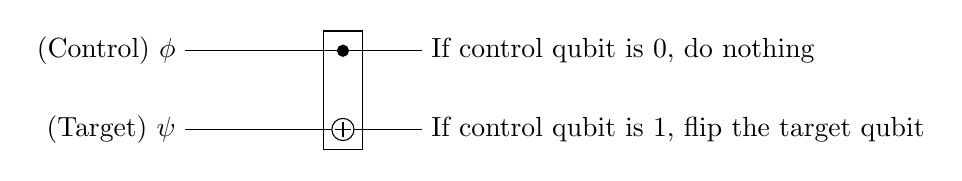
\begin{tikzpicture}
    
    \node [left] at (0, 1) {(Control) $\ket{\phi}$};
    \node [right] at (3, 1) {If control qubit is $\ket{0}$, do nothing};
    \node [left] at (0, 0) {(Target) $\ket{\psi}$};
    \node [right] at (3, 0) {If control qubit is $\ket{1}$, flip the target qubit};
    
    \draw (0, 1) -- (3, 1);
    \draw (0, 0) -- (3, 0);
    
    \filldraw [black] (2, 1) circle (2pt);
    \filldraw [draw=black, fill=white] (2, 0) circle (4pt);
    
    \draw (1.9, 0) -- (2.1, 0);
    \draw (2, -0.1) -- (2, 0.1);
    
    \draw (1.75, 1.25) -- (2.25, 1.25) -- (2.25, -0.25) -- (1.75, -0.25) -- cycle;
    
    \end{tikzpicture}
\end{center}

The next example on creating EPR states is intended to be a hands-on exercise to help you gain familiarity with tensor product manipulation.

\begin{example}[Creating EPR/Bell states]
To produce the EPR state $\ket{\Phi^+}:= \frac{1}{\sqrt{2}}(\ket{00} + \ket{11})$, we use a circuit consisting of a Hadamard gate ($H$) followed by a CNOT:
\begin{enumerate}
    \item \textbf{Initial State:} $\ket{\psi_0} = \ket{0} \otimes \ket{0} = \ket{00}$.
    \item \textbf{Apply $H$ to first qubit:} $\ket{\psi_1} = (H \otimes I)\ket{00} = \left(\frac{\ket{0} + \ket{1}}{\sqrt{2}}\right) \otimes \ket{0} = \frac{1}{\sqrt{2}}(\ket{00} + \ket{10})$.
    \item \textbf{Apply CNOT:} $\ket{\psi_2} = \text{CNOT} \left( \frac{1}{\sqrt{2}}(\ket{00} + \ket{10}) \right) = \frac{1}{\sqrt{2}}(\ket{00} + \ket{11})$.
\end{enumerate}

Diagrammatically,
    \begin{center}
        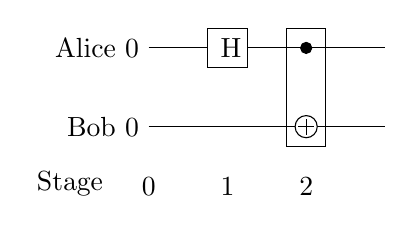
\begin{tikzpicture}
        
        \node [left] at (0, 1) {Alice $\ket{0}$};
        \node [left] at (0, 0) {Bob $\ket{0}$};

        \node [above] at (-1, -1) {Stage};
        \node [above] at (0, -1) {0};
        \node [above] at (1, -1) {1};
        \node [above] at (2, -1) {2};
        
        \draw (0, 1) -- (3, 1);
        \draw (0, 0) -- (3, 0);
        
        \filldraw [black] (2, 1) circle (2pt);
        \filldraw [draw=black, fill=white] (2, 0) circle (4pt);
        
        \draw (1.9, 0) -- (2.1, 0);
        \draw (2, -0.1) -- (2, 0.1);

        % H gate
        \draw [fill=white] (0.75, 1.25) -- (1.25, 1.25) -- (1.25, 0.75) -- (0.75, 0.75) -- cycle;
        \node [left] at (1.3, 1) {H};
        
        \draw (1.75, 1.25) -- (2.25, 1.25) -- (2.25, -0.25) -- (1.75, -0.25) -- cycle;
        
        \end{tikzpicture}
    \end{center}
\end{example}

\subsection{Quantum Entanglement}
Look at the Bell state again. We might think: what is the appropriate $\ket{\psi}$ and $\ket{\phi}$ such that $\ket{\Phi^+} = \ket{\psi} \otimes \ket{\phi}$? That is, what are the individual states of the qubits that collectively are described as the Bell state $\ket{\Phi^+}$ on the entire system?

Answer: there are no pairs of individual states $\ket{\phi}$ and $\ket{\psi}$ such that $\ket{\Phi^+} = \ket{\phi} \otimes \ket{\psi}$.
\begin{proof}
Assume that $\ket{\Phi^+} = \frac{1}{\sqrt{2}}(\ket{00} + \ket{11})$ is separable, i.e. there exist states $\ket{\psi} = \alpha_0\ket{0} + \alpha_1\ket{1}$ and $\ket{\phi} = \beta_0\ket{0} + \beta_1\ket{1}$ such that $$\ket{\Phi^+} = \ket{\psi} \otimes \ket{\phi}.$$

Expanding the tensor product out gives
\begin{align*}
\ket{\psi} \otimes \ket{\phi} &= (\alpha_0\ket{0} + \alpha_1\ket{1}) \otimes (\beta_0\ket{0} + \beta_1\ket{1}) \\
&= \alpha_0\beta_0\ket{00} + \alpha_0\beta_1\ket{01} + \alpha_1\beta_0\ket{10} + \alpha_1\beta_1\ket{11}
\end{align*}

We compare the coefficients of this expansion to the Bell state $\frac{1}{\sqrt{2}}\ket{00} + 0\ket{01} + 0\ket{10} + \frac{1}{\sqrt{2}}\ket{11}$:
\begin{enumerate}
    \item $\alpha_0\beta_0 = \frac{1}{\sqrt{2}}$ (from $\ket{00}$)
    \item $\alpha_0\beta_1 = 0$ (from $\ket{01}$)
    \item $\alpha_1\beta_0 = 0$ (from $\ket{10}$)
    \item $\alpha_1\beta_1 = \frac{1}{\sqrt{2}}$ (from $\ket{11}$)
\end{enumerate}

From (2), either $\alpha_0 = 0$ or $\beta_1 = 0$.
\begin{itemize}
    \item If $\alpha_0 = 0$, then $\alpha_0\beta_0 = 0$, which contradicts (1).
    \item If $\beta_1 = 0$, then $\alpha_1\beta_1 = 0$, which contradicts (4).
\end{itemize}

Since both possibilities lead to a contradiction, no such $\alpha_i, \beta_i$ exist. Therefore, $\ket{\Phi^+}$ is nonseparable.
\end{proof}

We say that $\ket{\Phi^+}$ is an \textbf{entangled} state. (Quantum) Entanglement is a \textit{core} feature of quantum mechanics and quantum computing, but mathematically it simply expresses the non-separability of the system state.

\begin{definition}[Separability and Entanglement]
Consider a composite quantum system described by the Hilbert space $\mathcal{H} = \mathcal{H}_A \otimes \mathcal{H}_B$. 
\begin{itemize}
    \item A pure state $\ket{\Psi} \in \mathcal{H}$ is said to be \textbf{separable} (or non-entangled) if it can be written as a tensor product of states from the individual subsystems:
    $$\ket{\Psi} = \ket{\psi}_A \otimes \ket{\phi}_B$$
    where $\ket{\psi}_A \in \mathcal{H}_A$ and $\ket{\phi}_B \in \mathcal{H}_B$.
    
    \item A pure state $\ket{\Psi}$ is said to be \textbf{entangled} if it cannot be decomposed in such a manner. That is:
    $$\ket{\Psi} \neq \ket{\psi}_A \otimes \ket{\phi}_B \quad \forall \ket{\psi}_A, \ket{\phi}_B$$
\end{itemize}
\end{definition}

While an entangled system state cannot be written as a tensor product of subsystem states, we \textit{can} actually make sense of and talk about these subsystem states, via the concept of partial trace. More on that later in the course.

\subsection{Partial Measurements}

So far we have seen how to describe composite systems and the operations on them, generally speaking. Performing measurements is also a type of operation. In this section we briefly explore the notion of partial measurements, i.e. making measurements only on a subsystem of the whole system.

Intuitively, if Alice measures \emph{only her qubit} in a joint state, she should obtain a classical outcome (here $0$ or $1$) according to the Born rule, and the \emph{post-measurement joint state} should be the part of the superposition consistent with that outcome, renormalized to have norm $1$.

Consider a general two-qubit state (Alice is the first qubit, Bob is the second):
\[
    \ket{\psi}
    = \alpha_{00}\ket{00}+\alpha_{01}\ket{01}+\alpha_{10}\ket{10}+\alpha_{11}\ket{11},
    \qquad
    \sum_{i,j\in\{0,1\}}|\alpha_{ij}|^2=1.
\]
Alice measures her qubit (in the computational basis). We have the case
\[
    \Pr[\text{Alice reads }\ket{0}] = |\alpha_{00}|^2 + |\alpha_{01}|^2
\]
wherein the state collapses to
\[
    \frac{\alpha_{00}\ket{00}+\alpha_{01}\ket{01}}{\sqrt{|\alpha_{00}|^2+|\alpha_{01}|^2}}
    = \gamma_0\ket{00}+\gamma_1\ket{01},
\]
where
\[
    \gamma_0=\frac{\alpha_{00}}{\sqrt{|\alpha_{00}|^2+|\alpha_{01}|^2}},
    \qquad
    \gamma_1=\frac{\alpha_{01}}{\sqrt{|\alpha_{00}|^2+|\alpha_{01}|^2}};
\]
and the case
\[
    \Pr[\text{Alice reads }\ket{1}] = |\alpha_{10}|^2 + |\alpha_{11}|^2
\]
wherein the state collapses to
\[
    \frac{\alpha_{10}\ket{10}+\alpha_{11}\ket{11}}{\sqrt{|\alpha_{10}|^2+|\alpha_{11}|^2}}
    = \gamma_0'\ket{10}+\gamma_1'\ket{11},
\]
where
\[
    \gamma_0'=\frac{\alpha_{10}}{\sqrt{|\alpha_{10}|^2+|\alpha_{11}|^2}},
    \qquad
    \gamma_1'=\frac{\alpha_{11}}{\sqrt{|\alpha_{10}|^2+|\alpha_{11}|^2}}.
\]
The amplitudes $\gamma_0,\gamma_1$ (respectively $\gamma_0',\gamma_1'$) are the \emph{conditional} probability amplitudes of the two-qubit basis states given Alice's outcome. Equivalently, they describe Bob's post-measurement state conditioned on Alice:
\[
    \ket{\psi_B \mid A=0}=\gamma_0\ket{0}+\gamma_1\ket{1},
    \qquad
    \ket{\psi_B \mid A=1}=\gamma_0'\ket{0}+\gamma_1'\ket{1},
\]
since in the $A=0$ branch the joint state is $\ket{0}\otimes(\gamma_0\ket{0}+\gamma_1\ket{1})$, and similarly for $A=1$.

Physically, Alice's measurement \emph{projects} the joint state onto the subspace consistent with her observed classical bit and the renormalization ensures the remaining state has total probability $1$. If $\ket{\psi}$ is a product state, measuring Alice does not change Bob's qubit. If $\ket{\psi}$ is entangled, then Bob's conditional state can depend on Alice's outcome, which is the source of the strong correlations observed in entangled measurements.

